\section{Работа с файлами}

\subsection{Условие задания}

Разработать приложение для своего варианта. 

Приложение должно содержать следующие компоненты:

\begin{enumerate}
    \item Заголовок формы должен отражать суть задания.
    \item Все элементы формы должны быть внятно подписаны (кнопки подписаны, у тестового поля должно быть написано, для чего оно нужно и т. д.)
    \item Структура представляет собой таблицу DataGridView, в ячейках которой записаны данные разных типов. 
    \item Предусмотреть кнопки: 
    \begin{itemize}
        \item считывание данных из файла и запись данных в таблицу (предполагается, что в файле данные корректные); 
        \item возможность добавлять и удалять строки в таблице, соответственно, вводить данные вручную.
        \item  запись в файл всех данных. Проверять корректность ввода данных: даты должны быть реальные, номер телефона состоять из цифр и, может быть, знак тире, оценки студентов - от 2 до 5. Все остальное можно не проверять. Если есть срок пребывания, дата прибытия и дата отбытия, то срок пребывания должен быть равен разнице между датой отбытия и датой прибытия.
        \item запись в файл данных по определенному критерию. Критерий можно вводить вручную через TextBox или выбирать c помощью Radiobox и т. д. Запись в файл должна быть такой, чтобы этот файл можно было открыть в приложении.
        \item запись данных по определенному критерию в новую таблицу. При выборе другого критерия старая таблица должна удаляться.
    \end{itemize}
    \item При неправильном вводе каких-либо данных таблица выбранных данных должна очищаться. 
    \item В коде должны быть комментарии и отступы (код должен быть легко читаем).
\end{enumerate}

\textbf{Вариант 11.} Создать таблицу \texttt{Travel}, содержащую следующие поля: Фамилия, имя, отчество туриста, название гостиницы, срок пребывания, дата приезда, дата отъезда. Выполнить следующие действия: считать из файла и вывести на экран данные о всех туристах, в другой файл вывести данные о туристах, приезжающих в данный день.

\subsection{Вид формы в конструкторе}


Создано окно приложения, содержащее один элемент TextBox, один элемент Label, шесть элементов Button, два элемента gridview,один элемент ErrorProvider для обработки ошибок и saveFileDialog и openFileDialog для работы с файлами. Вид окна представлен на рисунке \ref{task8_form} \cite{gladstone2022building}\cite{kaiser2022c++}.
\begin{figure}[H]
    \centering
    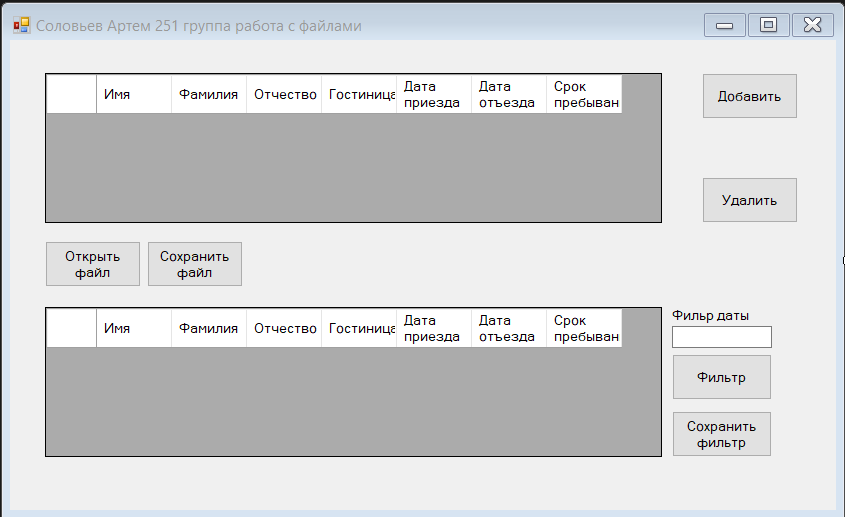
\includegraphics[width=1\linewidth]{lections/img/task8_form.png}
    \caption{Окно приложения «Матричный калькулятор» открытое в конструкторе}
    \label{task8_form}
\end{figure}


\subsection{Таблица с описанием переименованных элементов формы}
Все измененные элементы формы указаны в таблице \ref{task8_attributes}.


\begin{longtable}{|l|l|l|}
\caption{Значения атрибутов элементов в приложении <<Работа с файлами>>}\label{task8_attributes}\\
\hline
\textbf{\begin{tabular}[c]{@{}l@{}}Описание элементов\\ формы\end{tabular}}                         & \textbf{\begin{tabular}[c]{@{}l@{}}Список измененных\\ атрибутов\end{tabular}} & \textbf{\begin{tabular}[c]{@{}l@{}}Новое значение\\ атрибута\end{tabular}}             \\ \hline
\endfirsthead
%
\endhead
%
Форма MyForm                                                                                        & Text                                                                           & \begin{tabular}[c]{@{}l@{}}Соловьев Артем 251\\ группа работа с\\ файлами\end{tabular} \\ \hline
TextBox фильтра даты                                                                                & Name                                                                           & FilterDate                                                                             \\ \hline
\multirow{2}{*}{Кнопка "Добавить"}                                                                  & Name                                                                           & AddRow                                                                                 \\ \cline{2-3} 
                                                                                                    & Text                                                                           & Добавить                                                                               \\ \hline
\multirow{2}{*}{Кнопка "Удалить"}                                                                   & Name                                                                           & DeleteRow                                                                              \\ \cline{2-3} 
                                                                                                    & Text                                                                           & Удалить                                                                                \\ \hline
\multirow{2}{*}{Кнопка открытия файла}                                                              & Name                                                                           & FileOpen                                                                               \\ \cline{2-3} 
                                                                                                    & Text                                                                           & Открыть файл                                                                           \\ \hline
\multirow{2}{*}{Кнопка сохранения файла}                                                            & Name                                                                           & FileSave                                                                               \\ \cline{2-3} 
                                                                                                    & Text                                                                           & Сохранить файл                                                                         \\ \hline
\multirow{2}{*}{Кнопка фильтр даты}                                                                 & Name                                                                           & FilterBtn                                                                              \\ \cline{2-3} 
                                                                                                    & Text                                                                           & Фильтр                                                                                 \\ \hline
\multirow{2}{*}{\begin{tabular}[c]{@{}l@{}}Кнопка сохранить\\ отфильтрованную таблицу\end{tabular}} & Name                                                                           & FileSaveFilter                                                                         \\ \cline{2-3} 
                                                                                                    & Text                                                                           & Сохранить фильтр                                                                       \\ \hline
\multirow{2}{*}{Таблица постояльцев}                                                                & Name                                                                           & MainTable                                                                              \\ \cline{2-3} 
                                                                                                    & AllowUserToAddRows                                                             & False                                                                                  \\ \hline
\multirow{4}{*}{\begin{tabular}[c]{@{}l@{}}Таблица постояльцев\\ (отфильтрованная)\end{tabular}}    & Name                                                                           & FilteredTable                                                                          \\ \cline{2-3} 
                                                                                                    & AllowUserToAddRows                                                             & False                                                                                  \\ \cline{2-3} 
                                                                                                    & AllowUserToDeleteRows                                                          & False                                                                                  \\ \cline{2-3} 
                                                                                                    & ReadOnly                                                                       & True                                                                                   \\ \hline

\end{longtable}


\subsection{Примеры правильной и неправильной работы}
После запуска программы на экране появляется окно на рисунке \ref{task8_launch1}.
\begin{figure}[H]
    \centering
    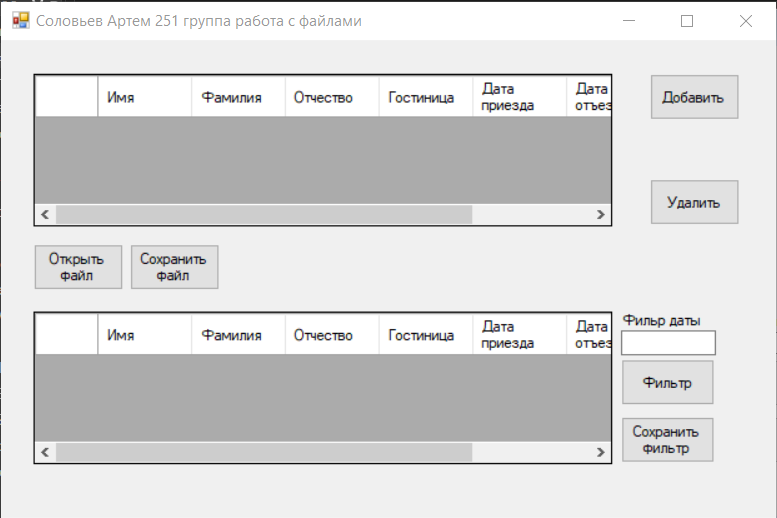
\includegraphics[width=0.8\linewidth]{lections/img/task8_launch1.png}
    \caption{Запуск программы}
    \label{task8_launch1}
\end{figure}

После ввода данных постояльцев, даты в фильтр даты и нажатии на кнопку "Фильтр" (на рисунке \ref{task8_launch2}).

\begin{figure}[H]
    \centering
    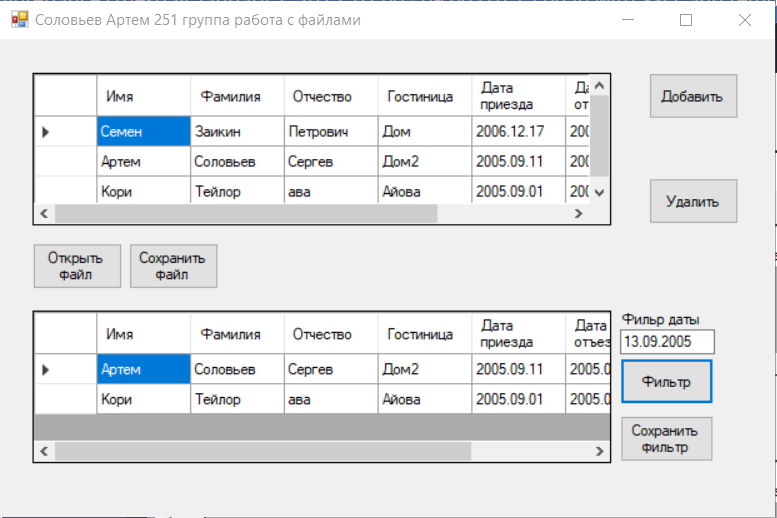
\includegraphics[width=0.8\linewidth]{lections/img/task8_launch2.png}
    \caption{Отфильтрованная таблица}
    \label{task8_launch2}
\end{figure}

При попытке ввода не даты в поле, программа выведет ошибку (на рисунке \ref{task8_launch3})
\begin{figure}[H]
    \centering
    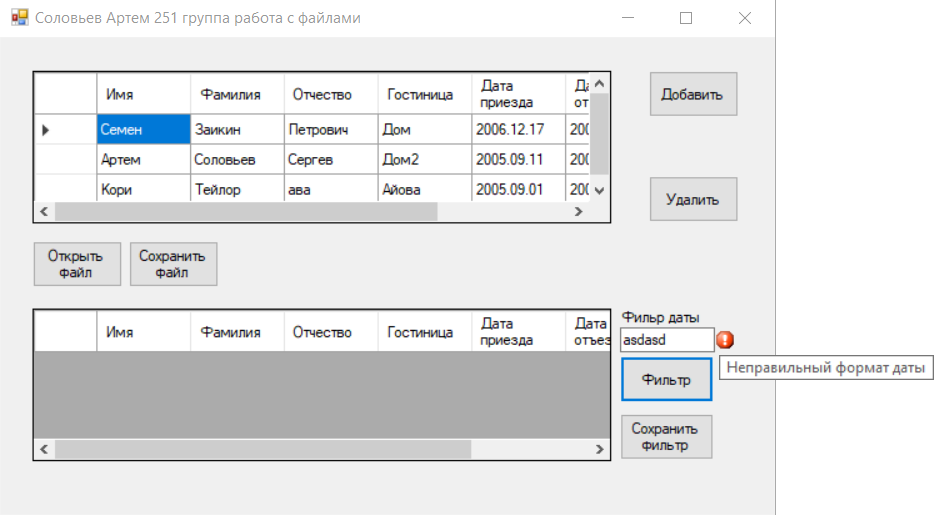
\includegraphics[width=1\linewidth]{lections/img/task8_launch3.png}
    \caption{Ошибка формата ввода}
    \label{task8_launch3}
\end{figure}


\subsection{Примеры исходного кода}


Функция удаления строки таблицы.
\begin{minted}[style=bw,
 linenos=true,
 breaklines=true,
 numbersep=5pt,
 tabsize=2,
 fontsize=\small,
 bgcolor=white]{cpp}
private: System::Void DeleteRow_Click(System::Object^ sender, System::EventArgs^ e) {
	this->errorProvider1->Clear();
	if (this->MainTable->RowCount == 0) {
		this->errorProvider1->SetError(DeleteRow, "Нельзя убрать строку, которой нет");
		return;
	}
	int i = this->MainTable->CurrentRow->Index;
	this->MainTable->Rows->Remove(this->MainTable->Rows[i]);
}
\end{minted}
Другие фрагменты кода расположены в приложении \ref{app:files}.

\sectionbreak